
\section{Auto-Vectorization}
\label{sec:autovec}

\subsection{Motivation}
The concept of applying operations to entire vectors of scalars can be called \textit{Array programming}. There
are languages like MATLAB, Ada, R or the \textbf{LLVM IR}  which support these kind of operations natively. 
Scalar languages like C, C++ or Java usually only work on simple scalar values.
\textbf{Vectorization} is the process of converting a scalar program into a program using vectors. 

\begin{figure}[H]
  \caption{Vectorization: Instead of sequential operations, the CPU processes data in parallel}
  \centering
    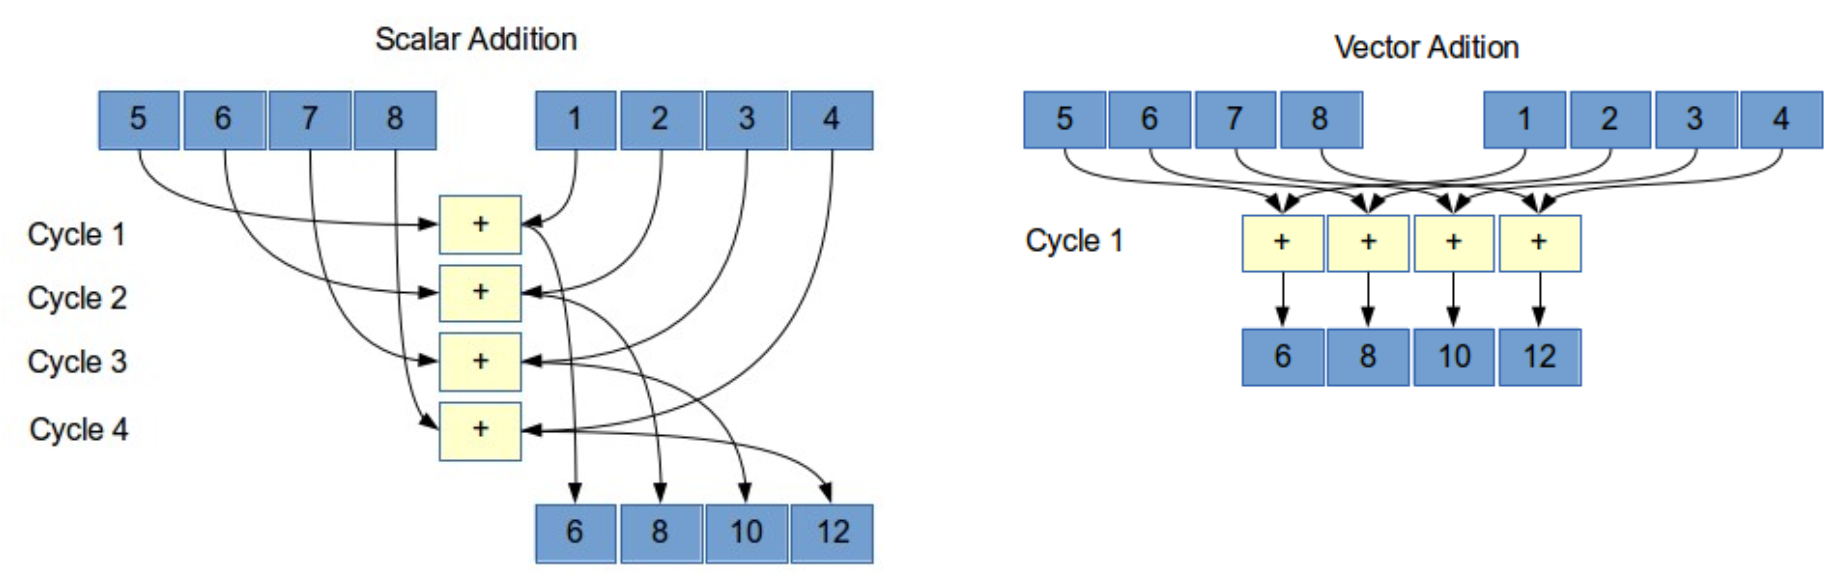
\includegraphics[width=\textwidth]{../slides/pictures/vectorization}
\end{figure}

CPU instructions working on vectors are commonly called \textbf{Single Instruction Multiple Data}. 
Most modern CPUs support SIMD instructions and have vector registers, with varying sizes. 
or example on modern x86 processors vector registers can have sizes of 128 (SSE), 256 (AVX2), 512 (AVX-512) bits.
Vectorization let's applications take advantage of these features to gain speed,
improve energy efficiency and have a smaller code base.


\subsection{Vectorization in LLVM}

As is evident now, there is a clear incentive for developers to use these SIMD instructions in their applications,
for computationally heavy tasks.
There exist language extensions (for example for C) to support vector operations, but this can be a complicated to use 
for the programmer. Additionally these language extensions are not necessarily cross-platform compatible.
Depending on the target architecture, the extension might work fine, other times it does not. 
For example consider this C program:
\begin{lstlisting}[language=C,label={lst:unvectorized}]
int a[8]; int b[8];
for (i=0; i < 8; i++)
    a[i] = a[i] + b[i];
\end{lstlisting}

Using the GCC vector extension (which works in LLVM too) we can rewrite this:
\begin{lstlisting}[language=C,label={lst:vectorization}]
// using 256bit AVX2 registers
typedef int vec8 __attribute__ ((vector_size (32)));
vec8 a, b;
a = a + b;
\end{lstlisting}
This is of course not necessarily desirable, to do manually. The size of the vector use might not actually be
available on the target platform. The code generator might need to legalize the vector operation, as described in
section~\ref{subsec:legalize}.

\subsection{Auto-Vectorization}

The compiler should be able to take care of vectorization for the developer.
The LLVM compiler is able to automatically vectorize certain code, if it fits certain criterias.
For vectorization the LLVM IR supports vector operations and data types natively. For example in this code
block we load two 8 element vectors with 32-bit integers from memory and multiply them:
\begin{lstlisting}[language=LLVM]
%vec1 = load <8 x i32>* %addr1
%vec2 = load <8 x i32>* %addr2
%vec3 = mul <8 x i32> %vec1, %vec2
\end{lstlisting}

The auto-vectorization poses a couple of challenges.
The data we want to work on must be in a format, which fits into the vector registers of the CPU.
Additionally the data must be correctly laid out in memory for the SIMD instructions.
The program behaviour must be preserved, otherwise a programmer couldn't rely on auto-vectorization.
The data dependencies in the program must be respected and the precision of the data types must stay the same.
If the precision would change, the program or behaviour output might change.

The LLVM compiler has two auto-vectorizers~\cite{llvm:vectorization}. These vectorizers focus on different kinds of codes 
and use different techniques. 
\begin{itemize}
\item The Loop Vectorizer, which only operates on Loops (for, while constructs)
\item SLP Vectorizer, which merges multiple scalars into vectors
\end{itemize}

\subsubsection{Loop Vectorizer}

The Loop Vectorizer rewrites loops to reduce the number of total operations.
The idea is to "widen" instructions which occur in the (innermost) loop body,
to operate on multiple consecutive iterations.

We previously saw an example of a loop~\ref{lst:unvectorized} which could be vectorized.
Using the C-lang vector extension we manually vectorized the code in~\ref{lst:vectorization}. If we would
want to do this with 512 entries in the vector, we can't just use a single addition of 4 integers anymore.
It is easy to determine that the 128-bit AVX registers can simultaneously compute on $128/32 = 4$ 32-bit integers.
Which means we only need a loop with $512 / 4 = 128$ iterations, instead of one with 512.
Using a (hyptothetical) variant of C, where arrays support a range syntax (similar to MATLAB) 
the vectorized loop would look something like this.
\begin{lstlisting}[language=C,label={lst:vectorized_loop}]
int a[512]; int b[512];
for (i=0; i < 512; i += 4)
    a[i:i+3] = a[i:i+3] + b[i:i+3];
\end{lstlisting}

The actual LLVM code was compiled with \lstinline[language=bash]{clang -O1 -S -emit-llvm}\\
The "-O1" option causes LLVM to only apply the loop vectorizer. For higher optimization levels the SLP vectorizer
will unroll the entire loop, to gain even more speed at the expense of having a bigger program size.
\begin{lstlisting}[language=LLVM]
vector.body: ; Loop body start
  %index = phi i64 [ %index.next, %vector.body ], [ 0, %3 ]
  ; The pointer arithmetic is omitted for %indexA/B
  ; loading vector of 4 integers, 
  %vec4A = load <4 x i32>, <4 x i32>* %indexA, align 16
  %vec4B = load <4 x i32>, <4 x i32>* %indexB, align 16
  ; computing the result
  %result = add nsw <4 x i32> %vec4A, %vec4B
  ; storing the result back into A
  store <4 x i32> %12, <4 x i32>* %indexA, align 16
  ; Compute the next index by adding 4
  %index.next = add i64 %index, 4
  ; check if the exit condition is met
  %exitcond = icmp eq i64 %index.next, 512
  br i1 %exitcond, label %middle.block, label %vector.body
\end{lstlisting}
If you read the code carefull, it becomes evident that LLVM generated code which is functionally equivalent
to the hypothetical vectorized C code~\ref{lst:vectorized_loop}.

\subsubsection{Compiler Hints}

The LLVM compiler supports extensions to hint the Loop vectorizer at possible
optimization opportunities. By interleaving the compiler stores multiple arrays interleaved in memory.
Sometimes this makes computations more efficent.
\begin{lstlisting}[language=C]
// The directive allows vectorization and interleaving to be enabled or disabled.
#pragma clang loop vectorize(enable) interleave(enable)
while(...) {
  ...
}
// Manually specify a vector width and interleaving count
#pragma clang loop vectorize_width(2) interleave_count(2)
for(...) {
  ...
}
\end{lstlisting}

\subsubsection{SLP Vectorizer}

The SLP Vectorizer can exploit possible parallelism of inline code in a code block. It combines
similar independent instructions into vector operations~\cite{conf/pldi/LiuZJDK12}. If configured it will check if unrolling
loops, will improve performance more than just vectorizing the loop body.
To find instruction patterns it uses the control flow graph and looks into basic blocks from the bottom-up 
for instructions to combine. Using this technique memory accesses, arithmetic operations, 
comparison operations and more can be vectorized.

The statements shown in figure~\ref{fig:slp_example} are identical (isomorphic).
They are parallized by a technique called \textit{statement packing}. 
\begin{figure}[H]
  \centering
    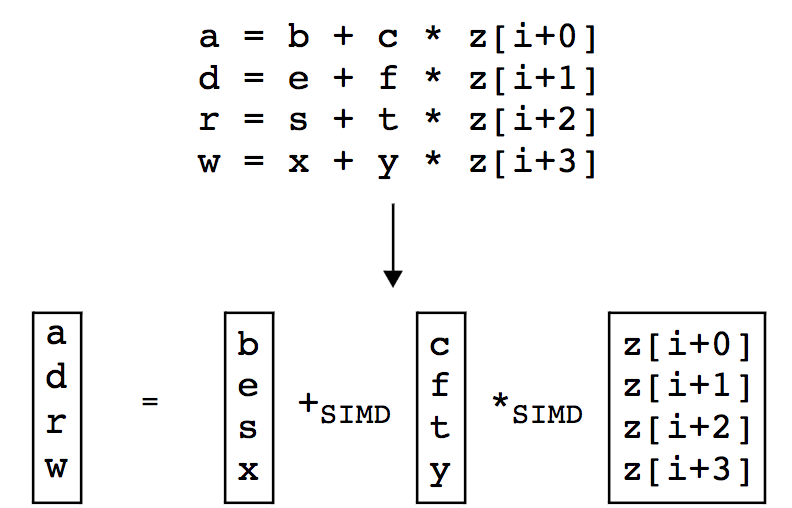
\includegraphics[width=.5\textwidth]{../slides/pictures/slp_example}
    \caption{Statements are contained in the same block and are structurally 
    identical(From~\cite{conf/pldi/LarsenA00})}\label{fig:slp_example}
\end{figure}
